\documentclass[crop,tikz]{standalone}

\usepackage{graphicx}
\usepackage{fancybox}
\usepackage{amsmath, amssymb}

\newcommand{\calP}{\mathcal{P}}
\newcommand{\bbR}{\mathbb{R}}
\DeclareMathOperator*{\argmax}{argmax}
\DeclareMathOperator*{\argmin}{argmin}

\usetikzlibrary{positioning}

\begin{document}

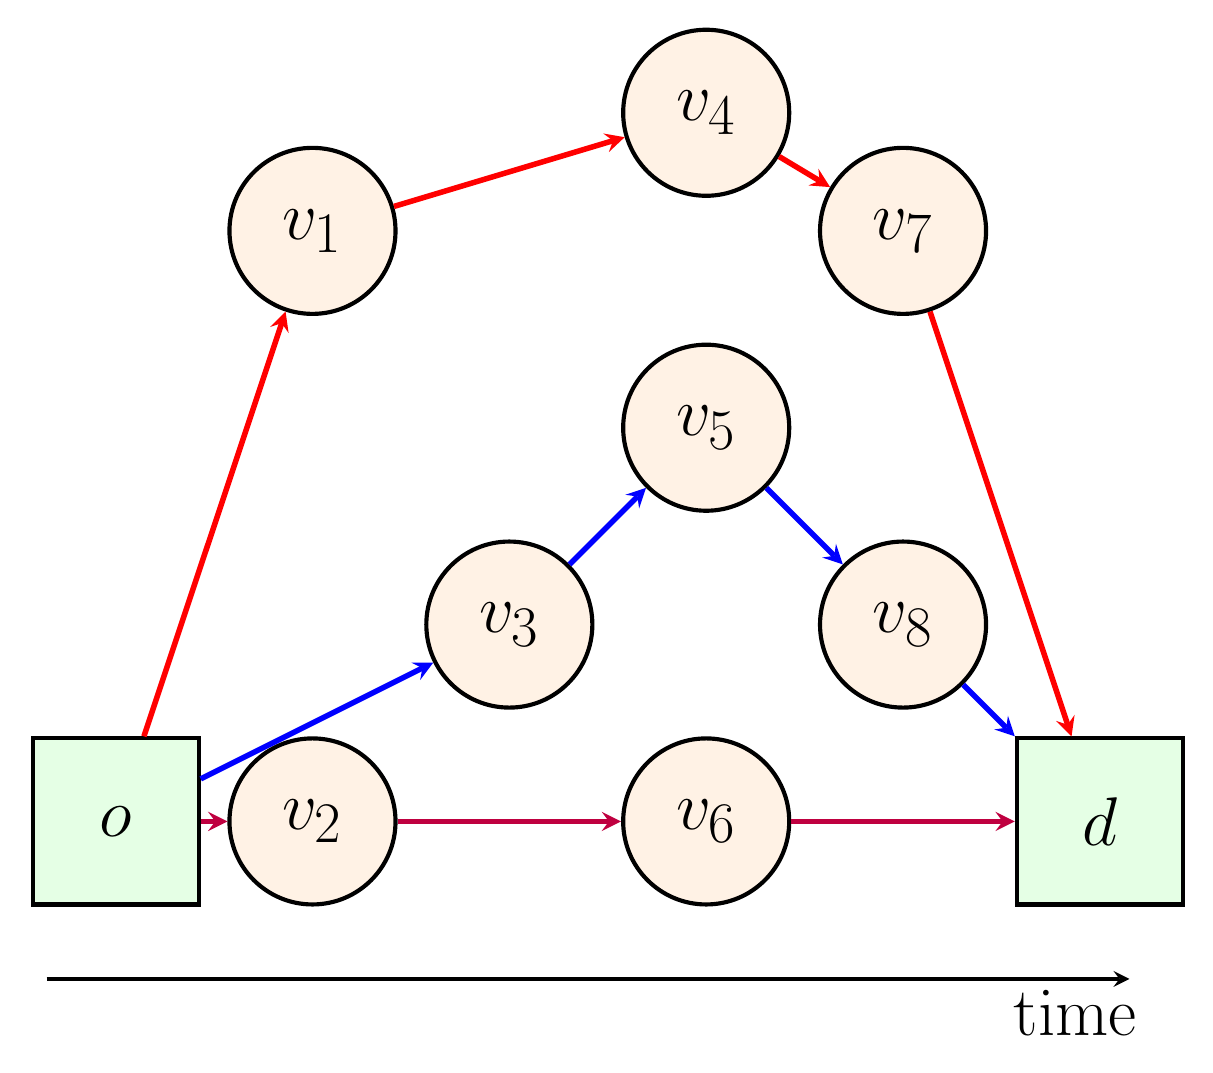
\begin{tikzpicture}

\tikzset{dummy/.style={fill=green!10, shape=rectangle, draw=black, minimum size=60, font=\Huge, line width=1.5}}
\tikzset{task/.style={fill=orange!10, shape=circle, draw=black, minimum size=60, font=\Huge, line width=1.5}}
\tikzset{selected/.style={->, >=stealth, line width=2}}
\tikzset{redpath/.style={selected, color=red}}
\tikzset{bluepath/.style={selected, color=blue}}
\tikzset{purplepath/.style={selected, color=purple}}
\tikzset{nopath/.style={thick, ->, dashed, line width=2}}
tikzset{EdgeStyle/.style = {
    thick,
    text = black,
    ->,>=stealth'
}}
\node[dummy] (o) at (0,0) {$o$};
\node[task] (v1) at (2.5,7.5) {$v_1$};
\node[task] (v2) at (2.5,0) {$v_2$};
\node[task] (v3) at (5,2.5) {$v_3$};
\node[task] (v4) at (7.5,9) {$v_4$};
\node[task] (v5) at (7.5,5) {$v_5$};
\node[task] (v6) at (7.5,0) {$v_6$};
\node[task] (v7) at (10,7.5) {$v_7$};
\node[task] (v8) at (10,2.5) {$v_8$};
\node[dummy] (d) at (12.5,0) {$d$};
\draw[redpath] (o) edge (v1);
\draw[redpath] (v1) edge (v4);
\draw[redpath] (v4) edge (v7);
\draw[redpath] (v7) edge (d);
\draw[bluepath] (o) edge (v3);
\draw[bluepath] (v3) edge (v5);
\draw[bluepath] (v5) edge (v8);
\draw[bluepath] (v8) edge (d);
\draw[purplepath] (o) edge (v2);
\draw[purplepath] (v2) edge (v6);
\draw[purplepath] (v6) edge (d);
% \draw[nopath] (v1) edge (v3);
% \draw[nopath] (v2) edge (v3);
% \draw[nopath] (v3) edge (v4);
% \draw[nopath] (v3) edge (v6);
% \draw[nopath] (v5) edge (v7);
% \draw[nopath] (v6) edge (v8);
\node[] (time1) at (-1, -2) {};
\node[] (time2) at (13, -2) {};
\draw[line width=1.5, ->, >=stealth] (time1) edge node[font=\Huge, below, pos=0.95]{time} (time2);

\end{tikzpicture}

\end{document}